\chapter{Membuat dan mengelola modul}
%script vs module: https://realpython.com/run-python-scripts/
\section{Pendahuluan}
\label{sec:awalmodul}
Modul dapat diartikan sebagai fungsi yang dapat dipanggil dari program Python apapun, selama lokasinya diketahui. Modul sangat berguna dalam menyederhanakan struktur aplikasi, sehingga setiap \textit{script} mengerjakan sedikit tugas utama yang saling terkait. Sedangkan tugas lain yang tidak terkait dipisahkan dalam \textit{script} yang bebeda di berkas yang berbeda. 

Perhatikan \lstlistingname~\ref{lst:faktorial} yang merupakan \textit{script} untuk menghitung nilai faktorial dari bilangan berjenis \texttt{int} yang dimasukkan. Faktorial, yang disimbolkan dengan \texttt{n!}, akan bernilai \texttt{n * n-1 * n-2 * $\ldots$ * 1}.

\lstinputlisting[language=python, numbers=left, numberstyle=\tiny, caption=Menghitung nilai faktorial, showstringspaces=false, label=lst:faktorial]{script/faktorial.py}

Jika perhitungan faktorial lebih dari satu kali, maka akan lebih efisien jika faktorial dibuat dalam fungsi tertentu yang dapat digunakan ulang tanpa menulis ulang. Perhatikan \lstlistingname~\ref{lst:faktorial2} di mana diperlukan dua kali pemanggilan terhadap fungsi \texttt{faktorial}. Dengan menerapkannya sebagai fungsi, kita tidak perlu menulis ulang fungsi \texttt{faktorial} (baris ke-1 s/d 8).

\pagebreak
\lstinputlisting[language=python, numbers=left, numberstyle=\tiny, caption=Menghitung nilai faktorial yang diterapkan sebagai fungsi, showstringspaces=false, label=lst:faktorial2]{script/faktorial2.py}

\section{Membuat modul}
Kita kembali ke kasus faktorial di sub bab \ref{sec:awalmodul}. Asumsikan jika ada beberapa \textit{script} yang membutuhkan fungsi \texttt{faktorial} tersebut. Maka, akan ada beberapa \textit{script} yang didalamnya terdefinisi fungsi \texttt{faktorial}. Pada kondisi inilah, modul memiliki peran penting. Perhatikan \lstlistingname~\ref{lst:faktorial3} yang penggunaannya memerlukan \textit{script} seperti \lstlistingname~\ref{lst:faktorialEks}.

\lstinputlisting[language=python, numbers=left, numberstyle=\tiny, caption=Fungsi faktorial sebagai modul, showstringspaces=false, label=lst:faktorial3]{script/faktorial3.py}

Maksud dari perintah di baris pertama \lstlistingname~\ref{lst:faktorialEks} adalah sebagai berikut.
\begin{itemize}
  \item \texttt{faktorial3} adalah nama file di mana modul faktorial didefinisikan (\texttt{faktorial3.py})
  \item \texttt{faktorail} adalah nama fungsi yang terdefinisi di modul faktorial
  \item \texttt{fk} adalah nama alias yang diberikan sebagai identitas fungsi \texttt{faktorial}. Fungsi dengan nama yang relatif panjang sering diberikan nama alias yang lebih singkat, terutama ketika fungsi tersebut sering digunakan
\end{itemize}

\lstinputlisting[language=python, numbers=left, numberstyle=\tiny, caption=\textit{Script} yang menggunakan modul \texttt{faktorial}, showstringspaces=false, label=lst:faktorialEks]{script/faktorialEks.py}

Pada kondisi lain, kita mungkin saja perlu melakukan pengujian terhadap modul yang kita bangun. Hal ini dapat disebabkan karena fungsinya kompleks sehingga selalu ada kemungkinan kesalahan dalam tahap pengembangannya. Maka, akan lebih mudah jika kita menyatukan \textit{script} yang bertugas untuk menguji dengan \textit{script} modul. Eksekusi terhadap \lstlistingname~\ref{lst:faktorial4} yang memanfaatkan modul seperti \lstlistingname~\ref{lst:faktorialEks2} akan menghasilkan luaran seperti pada \figurename~\ref{fig:modulUji}.

\lstinputlisting[language=python, numbers=left, numberstyle=\tiny, caption=Modul \texttt{faktorial} lengkap dengan fungsi ujinya, showstringspaces=false, label=lst:faktorial4]{script/faktorial4.py}

\lstinputlisting[language=python, numbers=left, numberstyle=\tiny, caption=\textit{Script} yang menggunakan modul \texttt{faktorial} yang di dalamnya ada fungsi uji, showstringspaces=false, label=lst:faktorialEks2]{script/faktorialEks2.py}

\begin{figure}
  \begin{center}
    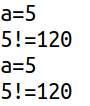
\includegraphics[scale=2.0]{pics/modulUji.png}
    \caption{Fungsi faktorial dipanggil dua kali}
    \label{fig:modulUji}
  \end{center}
\end{figure}

\figurename~\ref{fig:modulUji} menunjukkan bahwa fungsi \texttt{faktorial} dipanggil dua kali, masing-masing dari fungsi uji di luar modul dan fungsi uji di dalam modul. Untuk mengatasinya, perhatikan \lstlistingname~\ref{lst:faktorial5}. Dengan penambahan baris ke-8 di \lstlistingname~\ref{lst:faktorial5}, fungsi uji yang didefinisikan di modul tidak akan dieksekusi ketika modul tersebut sedang digunakan \textit{script} lain. \lstlistingname~\ref{lst:faktorial5} juga tampil lebih efisien dalam penulisan karena fungsi rekursif (pemanggilan fungsi itu sendiri) seperti ditunjukkan di baris ke-6.

\lstinputlisting[language=python, numbers=left, numberstyle=\tiny, caption=Modul \texttt{faktorial} lengkap dengan fungsi ujinya dan fungsi \texttt{main}, showstringspaces=false, label=lst:faktorial5]{script/faktorial5.py}
